\chapter{Synthesis of Verifiably Safe and Optimal Racing Maneuvers using Temporal Logic Specifications}
% \epigraph{\flushright The Pledge}{}
\epigraph{\flushright The first part is called "The Pledge". The magician shows you something ordinary \ldots he asks you to inspect it to see if it is indeed real, unaltered, normal. But of course... it probably isn't.}{Christopher Priest}
\label{chapter:synthesis}
\section{General Multi-Agent Racing Game Formulation} \label{section:genform}
To motivate our discretized game approximation, we begin by outlining a general multi-agent racing game formulation involving rules seen in real-life racing. 

% Table \ref{tab:gen_symbols} lists all of the variables and functions referenced in the formulation. 
Let there be a set, $N$, of players racing over $T$ steps in $\mathcal{T} = \{1, ..., T\}$. There is a track defined by a sequence of $\tau$ checkpoints along the center, $\{c_i\}_{i=1}^{\tau}$, whose indices are in a set $C=\{1,..., \tau\}$. The objective for each player $i$ is to minimize its pairwise differences of the time to reach the final checkpoint with all other players. In effect, the player targets to reach the finish line with the largest time advantage. The continuous state (such as position, speed, or tire wear) for each player, denoted as $x^i_t \in X \subseteq \mathbb{R}^n$, and control, denoted as $u^i_t \in U \subseteq \mathbb{R}^k$, are governed by known dynamics $f^i$. We also introduce a pair of discrete state variables $r^i_t \in C$ and $\gamma^i \in \mathcal{T}$. The index of the latest checkpoint passed by player $i$ at time $t$ is $r^i_t$, and it is computed by function $p: X\rightarrow C$. The earliest time when player $i$ reaches $c_\tau$ is $\gamma^i$. Using these definitions, we formulate the objective \eqref{eq:gen_obj} and core dynamics \eqref{eq:gen_dyn}-\eqref{eq:gen_goal_time} of the game as follows:

\begin{equation} \label{eq:gen_obj}
    \min_{u^i_0, ..., u^i_T} (|N|-1)\gamma^i - \sum^N_{j \neq i}\gamma^j \\
\end{equation}

\begin{equation} \label{eq:gen_dyn}
    x^j_{t+1} = f(x^j_t, u^j_t), \quad \forall \;\; t \in \mathcal{T}, j \in N
\end{equation}
\begin{equation} \label{eq:gen_idx_map}
    r^j_{t+1} = p(x^j_{t+1}, r^j_t), \quad \forall \;\; t \in \mathcal{T}, j \in N
\end{equation}
\begin{equation} \label{eq:gen_init_idx}
    r^j_{1} = 1, \quad \forall \;\; j \in N
\end{equation}
\begin{equation} \label{eq:gen_reach_goal}
    r^j_{T} = \tau, \quad \forall \;\; j \in N
\end{equation}
\begin{equation} \label{eq:gen_goal_time}
    \gamma^j = \min \{t \, | \, r^i_t = \tau \wedge t \in \mathcal{T} \}, \quad \forall \;\; j \in N
\end{equation}

In addition to the core dynamics of the game, there are rules that govern the players' states. To ensure that the players stay within the bounds of the track we introduce a function, $q: X \rightarrow \mathbb{R}$, which computes a player's distance to the closest point on the center line. This distance must be limited to the width of the track $w$. Therefore, for all $t \in \mathcal{T}$ and $j \in N$:
\begin{equation} \label{eq:gen_idx_dist}
    q(x^j_{t}) \leq w
\end{equation}

Next, we define the collision avoidance rules of the game. We use an indicator function that evaluates if player $i$ is ``behind" player $j$. Depending on the condition, the distance between every pair of players, computed by function the $D: X \rightarrow \mathbb{R}$, is required to be at least $s_1$ if player $i$ is behind another player $j$ or $s_0$ otherwise. Moreover, because following players have a greater collision avoidance responsibility than leading players, $s_1 \geq s_0$. For all $t \in \mathcal{T}$, $j \in N$, and $k \in N \setminus \{j\}$ these rules are expressed by the constraint:
\begin{equation} \label{eq:gen_coll_avoid}
    D(x^j_{t}, x^k_t) \geq  \begin{cases} s_1 & \mathds{1}_{\text{player} \, i \, \text{behind player}\,j} \\
    s_0 & \text{otherwise}  \end{cases}
\end{equation}

Finally, players are limited in how often they may change lanes depending on the part of the track they are at. We assume that there are $\lambda \in \mathbb{Z^+}$ lanes across all parts of the track. If the player's location on the track is classified as a curve, there is no limit on lane changing. However, if the player is at a location classified as a straight, it may not change lanes more than $L$ times for the contiguous section of the track classified as a straight. We define a set $\mathcal{S}$ that contains all checkpoint indices where a player is located at a straight section. We also introduce a function $z: X \rightarrow \{-1, 1, 2, ..., \lambda\}$ that returns the lane ID of a player's position on the track or $-1$ if the player is off-track. Using these definitions, we introduce a variable $l^j_t$ calculated by the following constraint for all $t \in \mathcal{T}$ and $j \in N$:
\begin{equation} \label{eq:gen_lane_var}
    l^j_{t} =  \begin{cases} l^j_{t-1} + 1 & \mathds{1}_{r^j_t \, \in \mathcal{S}} = \mathds{1}_{r^j_{t-1} \in \mathcal{S}}\wedge z(x^j_t) \neq z(x^j_{t-1}) \\
    0 & \text{otherwise}  \end{cases}
\end{equation}
This variable effectively represents a player's count of ``recent'' lane changes over a sequence of states located across a contiguous straight or curved section of the track. However, the variable is only required to be constrained if the player is on a straight section of the track. Therefore, the following constraint must hold for all $t \in \mathcal{T}$ and $j \in N$ and if $r^j_t \, \in \mathcal{S}$:
\begin{equation} \label{eq:gen_lane_lim}
    l^j_{t} \leq  L
\end{equation}
% Table of Symbols
% \begin{table} [!b]
% \centering
% \caption{Symbols in general formulation}
% \begin{tabular}{p{0.15\linewidth}|p{0.75\linewidth}}  \label{tab:gen_symbols}
% Symbol & Value\\ 
% \hline
% $N$ & Set of players in the game \\
% $\mathcal{T}$ & Set of steps in the game \\
% $\delta$ & Number of steps in the game \\
% $\{c_i\}_{i=1}^{\tau}$ & Sequence of checkpoints \\
% $C$ & Set of checkpoint indices \\
% $x^i_t$     &   Continuous state of player $i$ at time $t$   \\
% $u^i_t$      &   Control input of player $i$ at time $t$    \\
% $f(x^i_t, u^i_t)$  &  Continuous dynamics of player $i$ \\ 
% $r^i_t$      &  Index of last checkpoint passed by player $i$ at time $t$ \\ 
% $\gamma^i$     &  Time when player $i$ passed last checkpoint \\     
% $p(x^i_{t+1}, r^i_t)$  &  Function computing index of last track checkpoint passed  \\     
% $q(x^i_{t+1})$   &  Function computing minimum distance to last track checkpoint passed \\
% $w$      &  track width \\     
% $b^{(i,j)}_t$ & Binary state variable indicating if player i is directly behind player j \\
% $v(x^i_t, x^j_t)$ & Function computing value of $b^{(i, j)}_t$ \\
% $d(x^i_t, x^j_t)$ & Function computing distance between player i and player j \\
% $s_0$ & Minimum distance safety margin if player is not directly behind another \\
% $s_1$ & Minimum distance safety margin if player is directly behind another  \\
% $\lambda$ & Number of lanes in the track \\
% $l^i_t$ & Integer state variable indicating player $i$'s recent lane changes at time $t$ \\
% $y(x^i_t)$ & Function evaluating if player i is on a straight or curve \\
% $z(x^i_t)$ & Function computing the lane of the track player is in\\
% $L$ & Upper bound on the number of recent lane changes a player is allowed
% \end{tabular}
% \end{table}

% Describe challenges of special constraints -> better modeled as a discrete game
Most prior multi-agent racing formulations \cite{Wang2019, Wang2021, Li2021} do not include the complexities we introduced through defining constraints \eqref{eq:gen_coll_avoid}-\eqref{eq:gen_lane_lim}. They usually have a similar form regarding continuous dynamics and discrete checkpoints \eqref{eq:gen_dyn}-\eqref{eq:gen_goal_time}, and their rules only involve staying on track \eqref{eq:gen_idx_dist} and collision avoidance with a fixed distance. However, in real-life racing, there do exist these complexities both in the form of mutually understood unwritten rules and explicit safety rules \cite{racingrules}. As a result, we account for two of the key rules that ensure the game remains fair and safe:
\begin{enumerate}
    \item There is a greater emphasis on and responsibility of collision avoidance for a vehicle that is following another \eqref{eq:gen_coll_avoid}.
    \item The player may only switch lanes $L$ times while on a straight section of the track \eqref{eq:gen_lane_var}-\eqref{eq:gen_lane_lim}.
\end{enumerate}

The first rule ensures that a leading player can make a decision without needing to consider an aggressive move that risks a rear-end collision or side collision while turning from the players that are following. This second rule ensures that the leading player may not engage in aggressive swerving or ``zig-zagging" across the track that would make it impossible for a player that is following the leader to safely challenge for an overtake. 

While functions may exist to evaluate these spatially and temporally dependent constraints in the formulation, their discrete nature suggests that they cannot be easily differentiated. Therefore, it is not possible to simply apply state-of-the-art optimization algorithms would not apply to produce optimal control inputs in real-time. 

\section{Discrete Game Formulation}
In order to design a controller that can solve the realistic racing game formulation in the previous section, we must use an alternative to traditional optimization-based control methods. We recognize that complexities in the formulation arise from constraints over discrete properties of the players' trajectories. This characteristic of the formulation suggests that constructing a discrete abstraction of the game is an appropriate method to estimate feasible trajectories. In the following sections, we describe some abstractions and their justifications to construct a turn-based discrete game approximation of the original formulation. 

\subsection{Abstraction of State Space} \label{section:discstate}
We begin by constructing the discrete abstraction of the state space from the original formulation. We do not explicitly specify any components of players' states when defining the original formulation because it is agnostic to the vehicle dynamics model being considered. However, including variables computed by constraints \eqref{eq:gen_idx_map} and \eqref{eq:gen_lane_var}, we assume each player's state in the original game at least consists of following five variables as they are the only ones encoded in our discrete state representation:
\begin{itemize}
    \item position
    \item velocity
    \item number of ``recent" lane changes
    \item tire wear
    \item last passed checkpoint index
\end{itemize}
In the following subsections, we describe how the aforementioned state variables are transformed to produce a discrete model of a player.

\subsubsection{Discrete Representation of Racetrack}
\begin{figure}
\begin{center}
   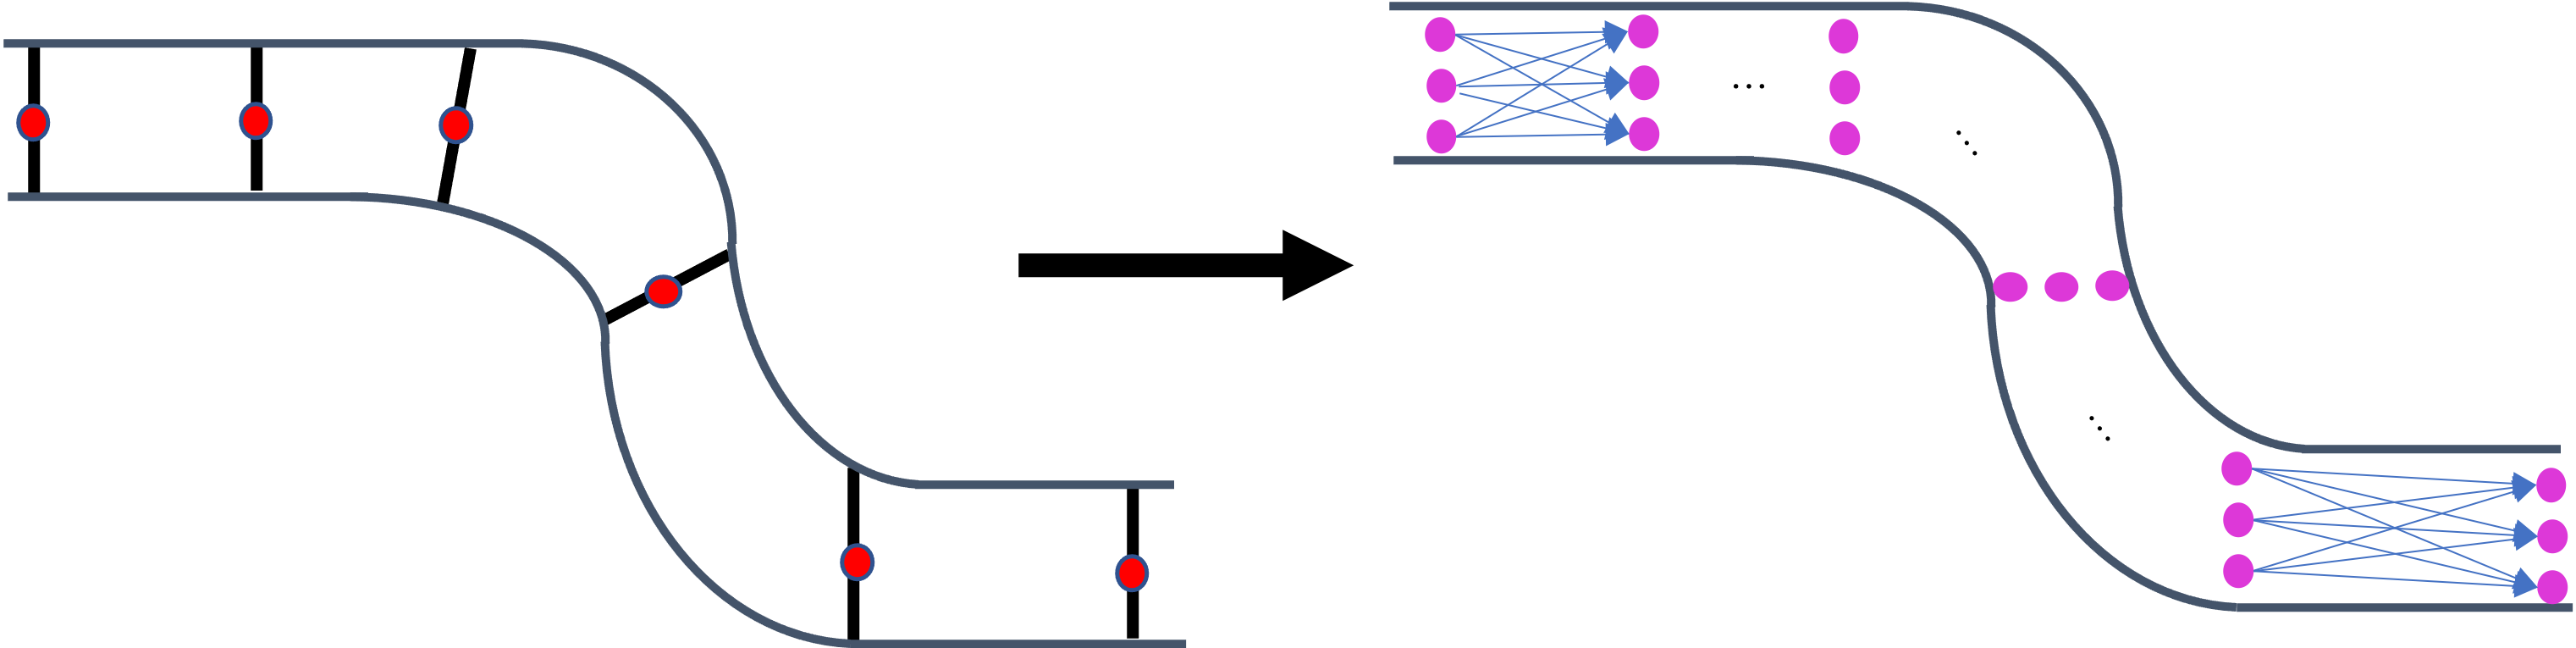
\includegraphics[width=\textwidth]{Figures/TrackAbstraction.png}
\caption[Transformation of racetrack in original formulation to discrete formulation.]{Transformation of the continuous race track with checkpoints (red) into discrete lanes at each checkpoint (purple).}
\label{fig:racetrack_abs}
\end{center}
\end{figure}
We change the mechanics so that the discrete game is played by making choices at the checkpoints that are indexed by $C$ rather than at each time-step from $\mathcal{T}$ defined in the original formulation. This transformation is natural to consider because all players must ultimately pass all checkpoints in order. As a result, the turns of the discrete game and players' states in the discrete game are indexed by their last passed checkpoint, and the time becomes a variable in the discrete game state. Furthermore, indexing by the checkpoints also produces a natural discretiziation for the position state variable in the original formulation. Around each checkpoint, we select $\lambda$ (which is the number of lanes) discrete locations along the line perpendicular to the direction of travel where each location evaluates to a unique lane ID on the track when passed into function $z(\cdot)$ defined in the general formulation. Therefore, we represent a player's position in discrete game formulation by its lane ID and index of the game state, i.e., the last passed checkpoint. This choice allows us to naturally encode the rules governing players' lanes and ensures that every location considered in the discrete game remains within the bounds of the track. Figure \ref{fig:racetrack_abs} visualizes the continuous space of the track with checkpoints (in red) is transformed into discrete locations associated with a unique lane ID at each checkpoint (in purple). 

\subsubsection{Discrete Representation of Player States}
\begin{figure}
\begin{center}
   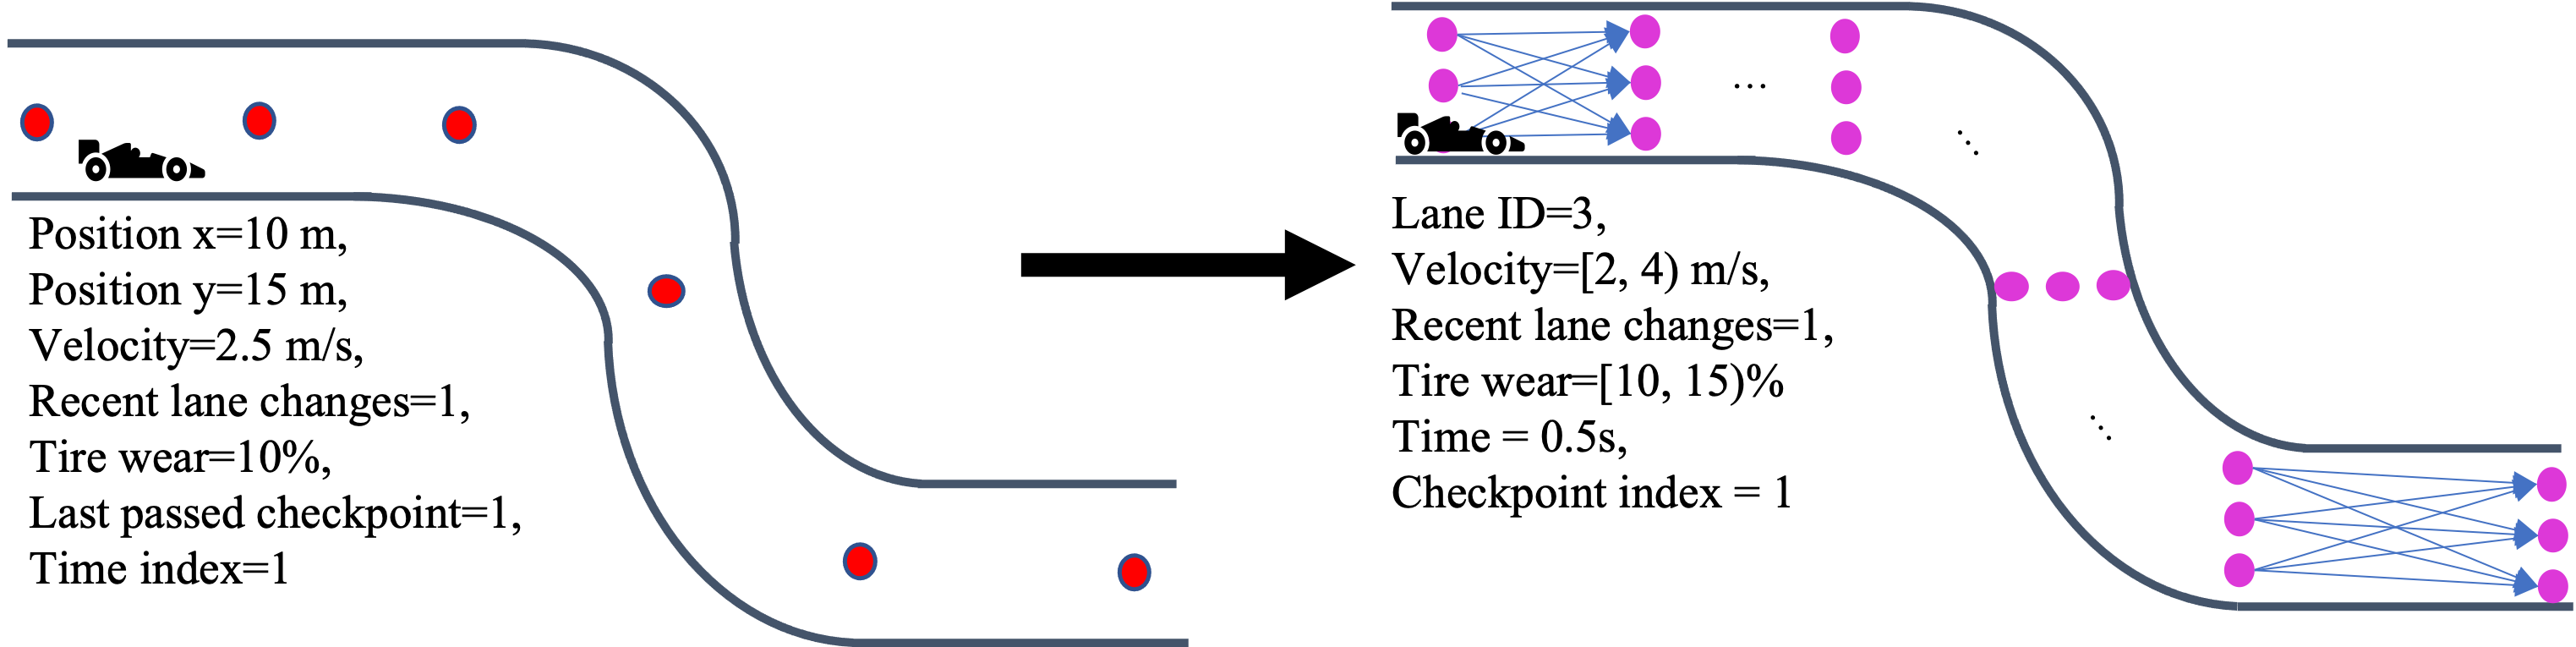
\includegraphics[width=\textwidth]{Figures/StateTransformation.png}
\caption{Transformation from original formulation state to discrete formulation state.}
\label{fig:state_transform}
\end{center}
\end{figure}
The remaining components of players' states are either already discrete valued, such as the count of ``recent lane changes," represented in the form of discrete buckets or rounded to a finite precision. For example, instead of considering real number value for a player $i$'s velocity from its state $x^i_v=\SI{2.5}{\meter\per\second}$ in the original game, the discrete representation would simply be $v^i \in [2, 4)\si{\meter\per\second}$. Figure \ref{fig:state_transform} visualizes a continuous state for a player converted into discrete form. The overall components of a player $i$'s discrete state are:
\begin{itemize}
    \item lane ID $a^i_k$
    \item velocity bucket $v^i_k$
    \item number of ``recent" lane changes $l^i_k$
    \item tire wear $e^i_k$
    \item time $t^i_k$
\end{itemize}
where $k$ is the index of the state and the checkpoint associated with the state. We also use the notation $k^i$ to refer to the index of the player $i$'s checkpoint in the overall game state because it is possible for the players' indices to be different as we are modeling a turn-based game.

\subsection{Abstraction of Dynamics} \label{section:discdyn}
Given discrete states of the players, we outline our abstraction of the dynamics, i.e. transitions between discrete states in the game. Because the discrete game is indexed by track checkpoint, we must also transform the players' control inputs. At each checkpoint, the players' choices are now the lane ID and target velocity bucket for the upcoming checkpoint. Next, we rewrite the constraints related to the racing rules in the original formulation as temporal logic specifications. We then discuss the specifics of how our state transitions are computed based on a given action and finish with describing the turn-based mechanism of the discrete formulation.

\subsubsection{Temporal Logic Specifications of Rules} 
Constraints regarding the rules of racing for player $i$ in the original transformation are now expressed as temporal logic specifications over the discretized state transformation:

\begin{enumerate}
    \item Stay on track \eqref{eq:gen_idx_dist}. To require that players stay on track we must ensure that the lane ID is within the subset of non-negative lane IDs.
    \begin{itemize}
        \item $\square \;  (a^i_k \in \{1, ..., \lambda\})$
    \end{itemize} 
    \item Avoid collisions \eqref{eq:gen_coll_avoid}. To abstract collisions, we require that players must always maintain a minimum time difference of $\mu$ if two players share the same lane ID at the same checkpoint. We assume that if there is a small time difference between the players at the same checkpoint and the same lane, there would be an increased risk of collision.
    \begin{itemize}
        \item $\square \;  ( \bigwedge_{j \in N \setminus i} (k^i=k^j \wedge a^i_k=a^j_k) \implies |t^i_k-t^j_k| \geq \mu))$
    \end{itemize}
    \item Limit lane changing on straights \eqref{eq:gen_lane_lim}. Ensure the ``recent" lane changes variable does not exceed $L$ if checkpoint index $k$ is a straight part of the track as represented by set $\mathcal{S}$ defined in the original formulation.
    \begin{itemize}
        \item $\square \; ((k \in \mathcal{S})  \implies (l^i_k \leq   L \; U \; k \notin \mathcal{S}))$
    \end{itemize} 
\end{enumerate}
The overall specification for each of the players is the conjunction of the list. Given our state discretization and action set, we could use synthesis methods to produce a controller to meet the specifications for some objective. However, the computational complexity of synthesizing a controller to meet such specifications is not manageable due to the exponential growth with respect to the number of specifications and variables \cite{Chen2013}. Therefore, we take advantage of the fact that most of these specifications are easily verified by simply examining a player's resulting state from a given state-action pair and that specification 1 is trivially satisfied by our state and action space abstraction (players are not allowed to choose target lanes outside of $\{1, ..., \lambda\}$). When constructing the model of the game, we simply disregard any player choice that violates the specifications thereby only considering states and trajectories that are allowed. 
\subsubsection{Computing State Transitions}
To check if a state-action pair satisfies the temporal logic specifications and the reasonably approximates vehicle dynamics, we must have a straightforward way of computing the resulting state variables when applying some action. 

Updating the lane ID and velocity states is trivial because it is the exactly the player's action. Similarly, updating the ``recent" lane changes variable is also simple with our state space design. We directly apply the logic from the original formulation \eqref{eq:gen_lane_var}. It only requires evaluating whether the track type classification of the pair of checkpoints is the same and if the choice of lane ID is different than the lane ID at the initial checkpoint. Therefore, if choosing an action implies that lane change limit $L$ is exceeded on the straight checkpoints, the action would be disregarded in model to satisfy specification 3. 

To calculate updates for the elapsed time state, we first use the known track parameters (such as turning radius or lane width) to estimate the distance to travel between the lane in the current checkpoint $c_k$ to the lane in the subsequent checkpoint $c_{k+1}$. If the track between two checkpoints is a straight, the Euclidian is used to estimate the distance to travel based on the lane width ($w_l$) and the distance between the location of the checkpoints $\gamma_{k, k+1}$. If the the track between the two checkpoints is a curve, then we calculate a coarse estimate of the distance by averaging the radius of the turn for player's lane at the initial checkpoint $r_k$ and radius of the turn for the player's target lane at next checkpoint $r_{k+1}$ and multiply it by the central angle of the turn $\theta_k$. These calculations are summarized below:

\begin{equation} \label{eq:dist_calc}
    d = \begin{cases}
    \sqrt{w_l^2 + \gamma_{k, k+1}^2} &  \text{if } k \in \mathcal{S} \\
    \frac{r_k + r_{k+1}}{2}\theta_k & \text{if } k \notin \mathcal{S}
    \end{cases}
\end{equation}

Given the estimated distance $d$, average velocity of bucket at the initial checkpoint $\bar{v}_k$ and average velocity of the target bucket $\bar{v}_{k+1}$ and parameters of the vehicle such as maximum allowed velocity $v_*$, maximum acceleration $a$, and maximum braking $b$, we use simple equations of motion to calculate minimum time it takes to travel the distance.  Moreover, maximum allowed velocity $v_*$ is estimated using the tire wear state at the initial checkpoint $e_k$, track radius, and the parameter of a vehicle's maximum allowed lateral acceleration. We enforce that $\bar{v}_{k+1} \leq v_*$ and disregard all actions that violate this requirement because such an action would not obey the lateral acceleration limitation of the vehicle. In addition, we verify it is possible to accelerate or decelerate from $v_k$ to $v_{k+1}$ within the distance if $v_k \leq v_{k+1}$ or $v_k \geq v_{k+1}$, respectively. If that is not possible, then the action with target velocity $v_{k+1}$ is also disregarded. For the remaining cases, we use the following calculation for the time update $\delta t_k$:

\begin{equation} \label{eq:time_update}
    \delta t_{k} = \begin{cases}
    \frac{v_*-\bar{v}_k}{a} + \frac{v_*-\bar{v}_{k+1}}{b} + \frac{d-\frac{v_*^2-\bar{v}_k^2}{2a} - \frac{v_*^2-\bar{v}_{k+1}^2}{2b}}{v_*} 
    &  \text{if } v_* \geq \bar{v}_k \; \wedge \\
     &\quad \frac{d-\frac{v_*^2-\bar{v}_k^2}{2a} - \frac{v_*^2-\bar{v}_{k+1}^2}{2b}}{v_*} \geq 0 \\
    \frac{\bar{v}_k -v_*}{b} + \frac{v_*-\bar{v}_{k+1}}{b} + \frac{d-\frac{\bar{v}_k^2 -v_*^2}{2b} - \frac{v_*^2-\bar{v}_{k+1}^2}{2b}}{v_*} 
    &  \text{if } v_* < \bar{v}_k \;\wedge \\
    &\quad \frac{d-\frac{\bar{v}_k^2 -v_*^2}{2b} - \frac{v_*^2-\bar{v}_{k+1}^2}{2b}}{v_*} \geq 0 \\
    \frac{\sqrt{\frac{-2dba -b\bar{v}_k^2 -a\bar{v}_{k+1}^2}{-a-b}}-\bar{v}_{k}}{a} + \frac{\sqrt{\frac{-2dba -b\bar{v}_k^2 -a\bar{v}_{k+1}^2}{-a-b}}-\bar{v}_{k+1}}{b}
    & \text{if } \bar{v}_k \leq v_* \\
    \text{action ruled out}
    & \text{otherwise}
    \end{cases}
\end{equation}

The calculation simply assumes the player accelerates or brakes to reach $v_*$ from $\bar{v}_k$, maintains that speed for as long as possible until the player must brake to hit $\bar{v}_{k+1}$ if $\bar{v}_{k+1} \neq v_*$. If there is not enough distance to perform this maneuver and $\bar{v}_k \leq v_*$, we calculate the highest velocity the player can hit given we must end at the target velocity within the specified distance. All other possible maneuvers would violate the dynamical limitations of the vehicle and are ruled out of the allowed actions. We also use the time state update to estimate collision avoidance and satisfy specification 2. If a player chooses a lane that a prior player has already selected for its turn and the difference in the time states for these players would be smaller than $\mu$ if the action is applied, then the action is disregarded.

Finally, in order to calculate the tire wear state update, we consider the straight and curve differently. If the track between the checkpoints is a straight, we multiply a tire wear factor parameter $L_{\text{straight}}$ for a straight with the distance of the straight $d$. When the track between the checkpoints is a curve, we multiply the tire wear factor parameter $L_{\text{curve}}$, the distance of the curve $d$, and an estimate for the average lateral acceleration achieved by hitting the target velocity $\bar{v}_{k+1}$ calculated using equations of circular motion. The tire wear update $\delta e_k$ is calculated as follows:
\begin{equation}
\delta e_k = \begin{cases}
    dL_{\text{straight}} & \text{if } k \in \mathcal{S} \\
    \frac{2dL_{\text{curve}}\bar{v}_{k+1}^2}{r_k + r_{k+1}} & \text{if } k \notin \mathcal{S}
\end{cases}
\end{equation}
For both the time and tire wear, the updates are added to the initial state and projected back into their discrete buckets or rounded to the finite precision.

Using these calculations, we have a way of computing the exact sequence of states given a sequence of player actions. Next, we discuss the final piece of our discrete game's dynamics by outlining the logic behind determining the order in which the players choose actions. 

\subsubsection{Turn-Based Mechanics}
Although players make decisions concurrently in the original game and real-life, our discrete abstraction is a modeled as a turn-based game. Because the states are indexed by the checkpoint instead of time, the game is played by evaluating the choices all players one checkpoint at a time. The order in which the players choose their actions at each checkpoint is determined by the player who has the smallest time state at the checkpoint being processed. A lower time state value implies that a player was at the given checkpoint before other players, so it would have made its choice at that location before the others in the continuous setting. This ordering also implies that players who arrive at a checkpoint after preceding players observe the actions of those preceding players preserving the realistic flow of information. Most importantly, because the ordering forces the following players to choose last, we also capture the rule that the following players (i.e. those that are ``behind'' others) are responsible for collision avoidance after observing the leading players' actions. As a result, in conjunction with satisfying specification 2, we model realistic collision avoidance rules. 

\subsection{Discrete Game Objective} \label{section:discobj}
The final component of our discrete game is the determining the rewards and the objective. The reward function for a player $i$ is: 
\begin{equation}
    R^i(s^1, ... s^n) = \begin{cases} 
                (\sum_{j \in N \setminus i} s^j_t) - |N-1|s^i_t & (\bigwedge_{m \in N} s^m_k   = c_\tau) \\ 
                0    & \quad \text{otherwise}
                \end{cases}
\end{equation}
It is zero for all states except the one after all players have reached the final checkpoint. At the final checkpoint, player $i$'s reward is the pairwise difference in the time state with each player after everyone has reached the goal, which resembles the original game formulation's objective \eqref{eq:gen_obj}. The objective for each player is to simply maximize this reward.

\subsection{Summary of Formulation}
Given the state space, dynamics, and objective of the game, we have effectively constructed a finite dynamic game. We write this game in a more general form as a stochastic multiplayer game (SMG) defined by Chen et al. as a tuple of the following elements \cite{Chen2013}:


\begin{itemize}
    \item $S$ is the finite state space of the game, which is the set product of all players and the domains of each of the state variables.
    \item $A^1(\boldsymbol{s}), \ldots, A^{|N|}(\boldsymbol{s})$ are the finite action sets of each of the players dependent on the current state, which includes full knowledge of the other player' state and the track position variable.
    \item $F^1(\boldsymbol{s}, a^1, \boldsymbol{s}'), \ldots, F^{|N|}(\boldsymbol{s}, a^{|N|}, \boldsymbol{s}')$ are the transition functions for each player following the calculations described previously.
    \item $R^1(\boldsymbol{s}),\ldots,R^{|N|}(\boldsymbol{s})$ are the reward functions provided in the prior section.
     \item $AP = \{\text{goal}\}$ atomic propositions.
    \item $L: S \rightarrow 2^{AP}$ is the labeling function for the states for the set $AP$. The function labels all states where all players have reached the final checkpoint with $\{\text{goal}\}$, and all other states with $\varnothing$.
\end{itemize}

Once in the SMG form, we can use state-of-the-art model checking tools with a simple reachability specification, $\lozenge \text{goal}$, to synthesize optimal strategies for the players to maximize their rewards. 
% Furthermore, we are guaranteed to find a pure strategy Nash equilibrium because we constructed a finite dynamic game. CITETHIS\footnote{\url{https://econ.uiuc.edu/~hrtdmrt2/Teaching/GT_2017_19/L3.pdf}}.

\section{Case Studies of Strategic Scenarios}
\begin{figure}
\begin{center}
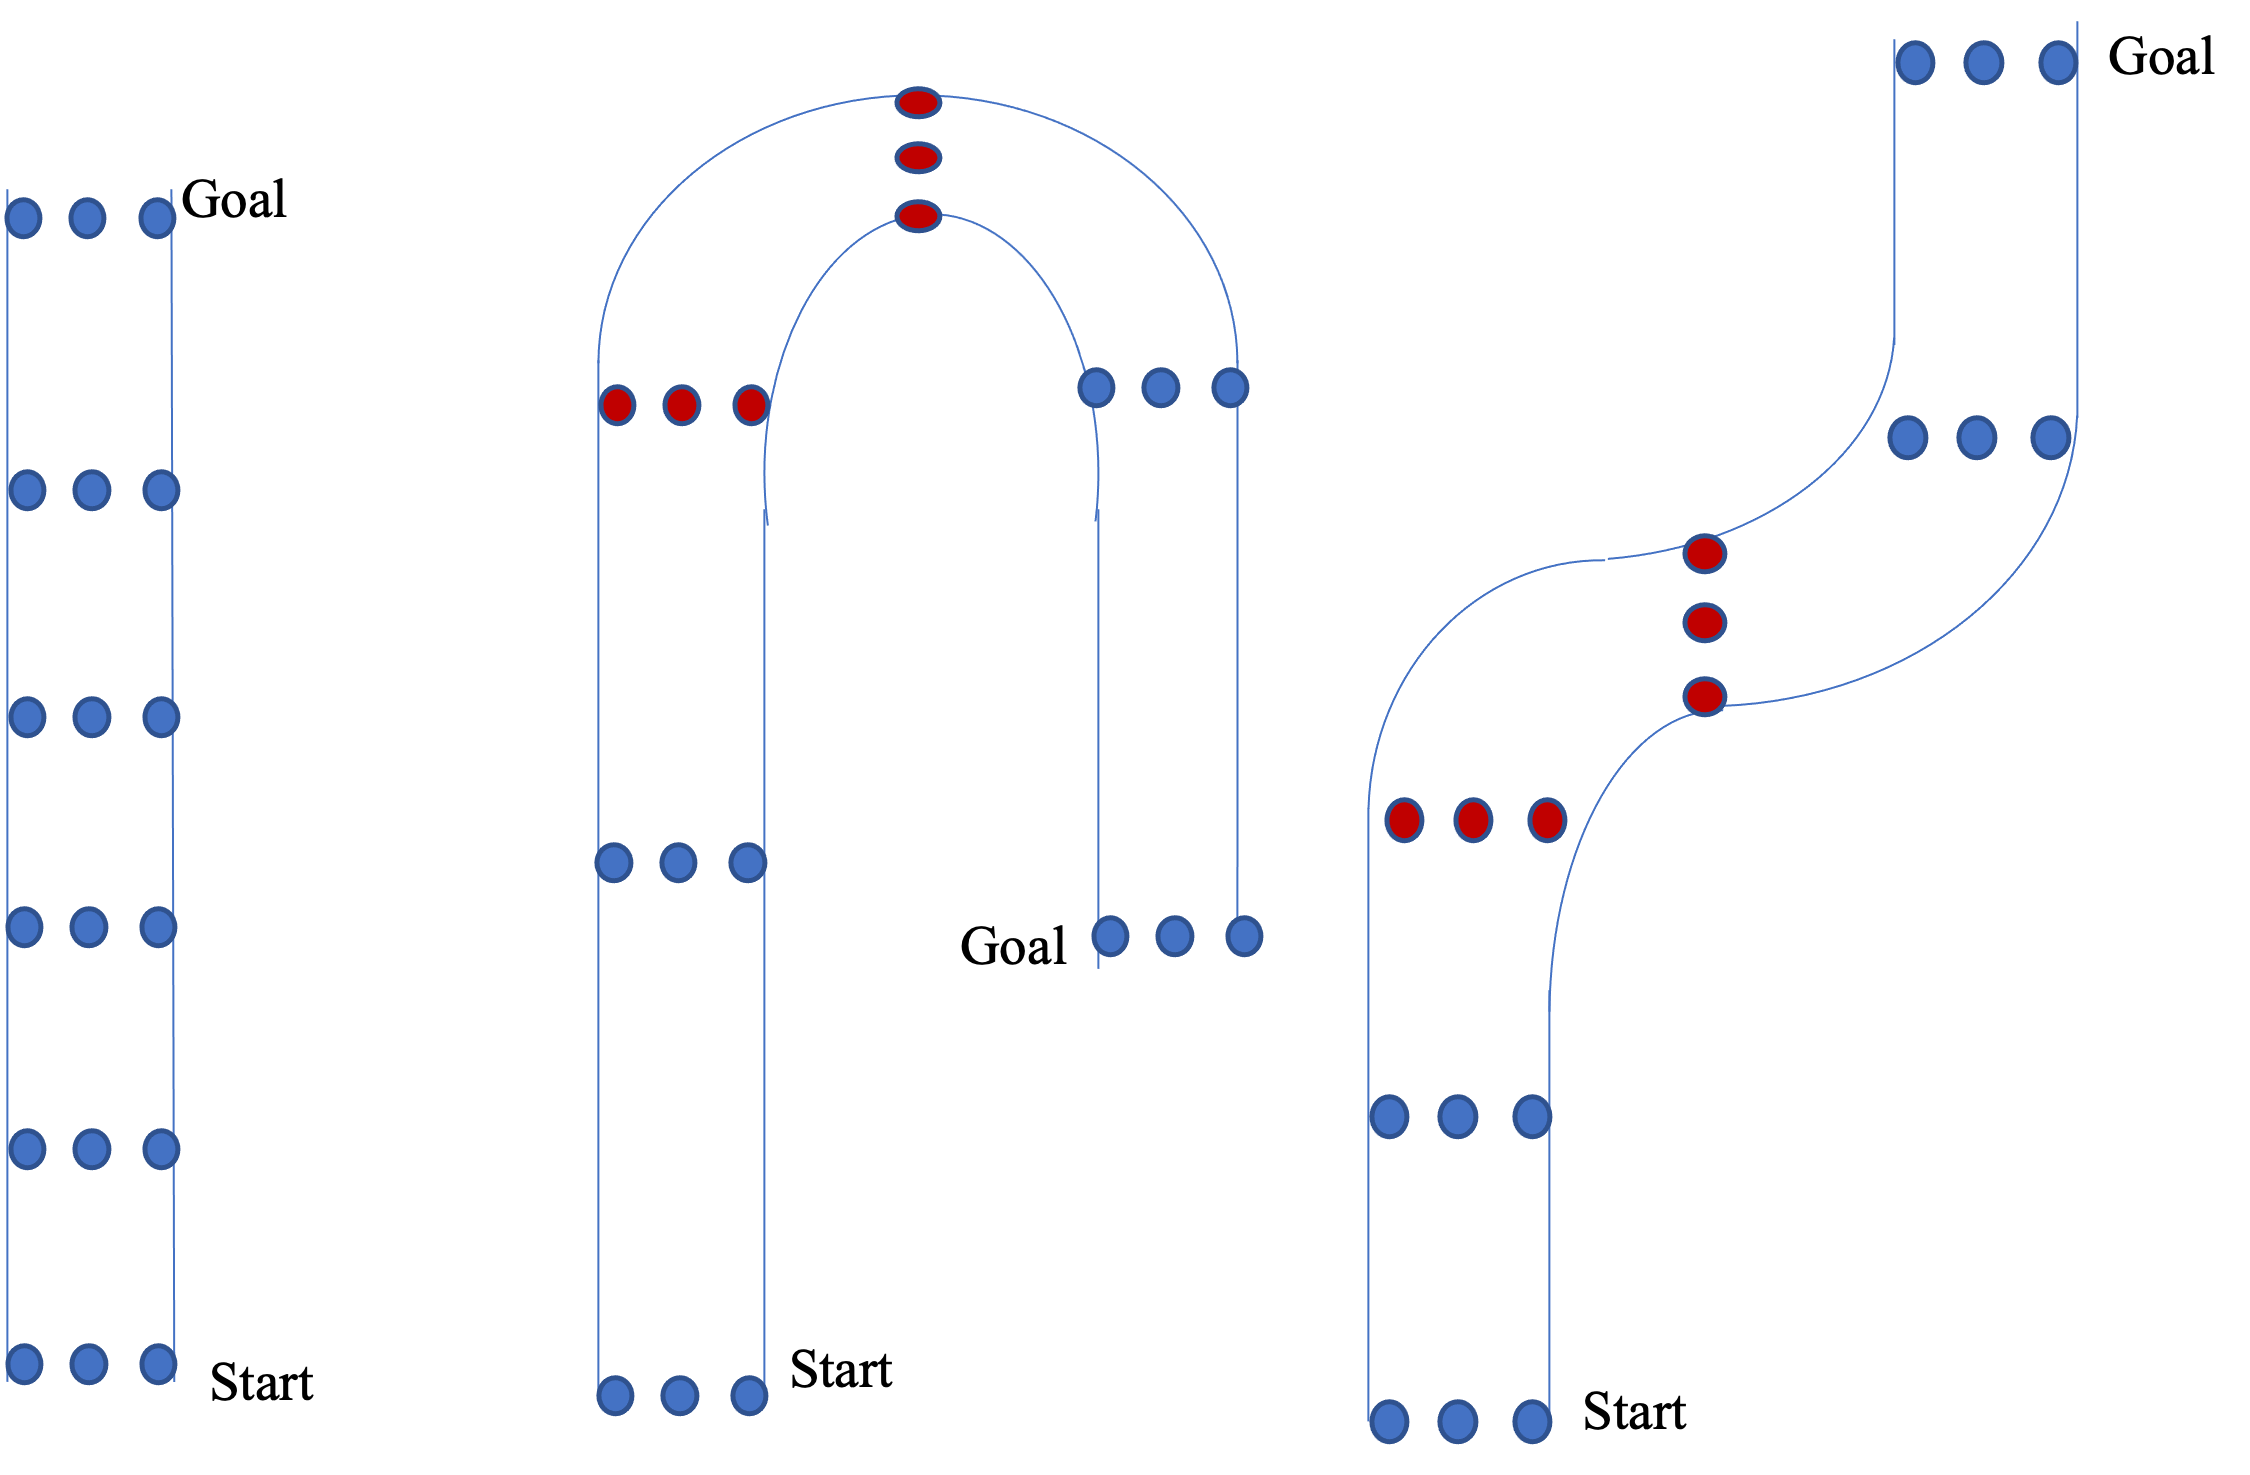
\includegraphics[width=\textwidth]{Figures/TrackShapes.png}
    \caption[Discrete representation of common track shapes.]{\label{fig:track_shapes} Three track types straight, hairpin, and chicane visualized from left to right. Each shape is discretized by 6 checkpoints and 3 lanes. The discrete nodes are color coded using their classification as straights (blue) or corners (red).}
\end{center}
\end{figure}
To evaluate if our discrete game formulation is a reasonable representation of real-life racing, we apply the model to several case studies resembling some common race scenarios for two players. The goal is to visualize and interpret the produced strategies to ensure it matches with our prior understanding of what might happen in a similar scenario in real-life racing. We categorize the scenarios based on three common types of track shapes: long straight, hairpin, and chicane shown in Figure \ref{fig:track_shapes}. For each of the track shapes, we explore various combinations of initial states for tire wear, velocity, and elapsed time for the players. We analyse the scenarios in the perspective of player 1 and start it with a non-zero time state for each study. Setting a non-zero initial time state indicates that it is starting with a disadvantage and is behind player 2. However, we analyze the initial states where player 1 is able to overtake player 2 or see what the best time gap it achieves. 

In order to make the results of the studies more interesting, we also assume that the players' vehicles have different dynamical parameters. Player 1 has a higher top speed than racer 2 but has a lower acceleration than racer 2. However, racer 2 has a higher limit for maximum lateral acceleration, which is used for computing maximum velocity allowed during turning, but it also has a higher tire wear factor. If both cars have the exact same configuration, the strategies of both vehicles would be similar. Furthermore, it would be near impossible for the player 1 to overtake the player 2 with perfect play. The exact parameters used when generating the transitions functions for each player is listed in Table \ref{table:params}.

\begin{table}
\resizebox{\textwidth}{!}{%
\begin{tabular}{|l|l|l|}
\hline
\textbf{Vehicle Parameter}                                                                                                 & \textbf{Player 1} & \textbf{Player 2} \\ \hline
Maximum velocity (\si{\meter\per\second})                                                                                            & 7       & 6       \\ \hline
Maximum longitudinal acceleration (\si{\meter\per\second\squared})                                                         & 3       & 4       \\ \hline
Minimum longitudinal acceleration, i.e. maximum braking force (\si{\meter\per\second\squared})                                                         & -4      & -4      \\ \hline
Maximum lateral acceleration (\si{\meter\per\second\squared})                                                             & 5.88    & 6.86    \\ \hline
Minimum lateral acceleration (force that can be sustained regardless at any tire wear state)  (\si{\meter\per\second\squared}) & 2.94    & 2.94    \\ \hline
\end{tabular}%
}
\caption{Parameters used to generate transitions for the model tested in the case study scenarios.}
\label{table:params}
\end{table}

For the results in each case, we plot the ``best" time gap player 1 achieves assuming optimal strategy is implemented by both the players. If this value is positive, it means player 1 has reached the goal position before player 2 and vice-versa if negative. All of the models are implemented using PRISM-games v3.0, a state-of-the-art model checking software \cite{prismgames}. Furthermore, our analysis for each track shape includes a visualization plotting the optimal strategy and comparison of the resulting strategy to a similar, real-life racing scenario. This comparison allows us to verify that the strategic choices of our model synthesis are comparable to human experts. 

\subsection{Long Straight}
The first track shape is the simple long straight. In this case, tire wear has little to no effect on the performance of the players because the vehicles are not subject to significant lateral loads. Rather, we know from real-life races that we can having advantage in the initial time gap or higher initial speed when approaching the long straight results in a favorable time gap at the end of the straight. Therefore, we experiment with various initial velocities and time gaps between the players. Player 1's initial value of the time state, i.e. time disadvantage, varies from \SI{0.5}{\second} to \SI{0.7}{\second}. However, player 1's initial speeds may be higher in some experiments yielding the possibility of an overtake.

\begin{figure}[t!]
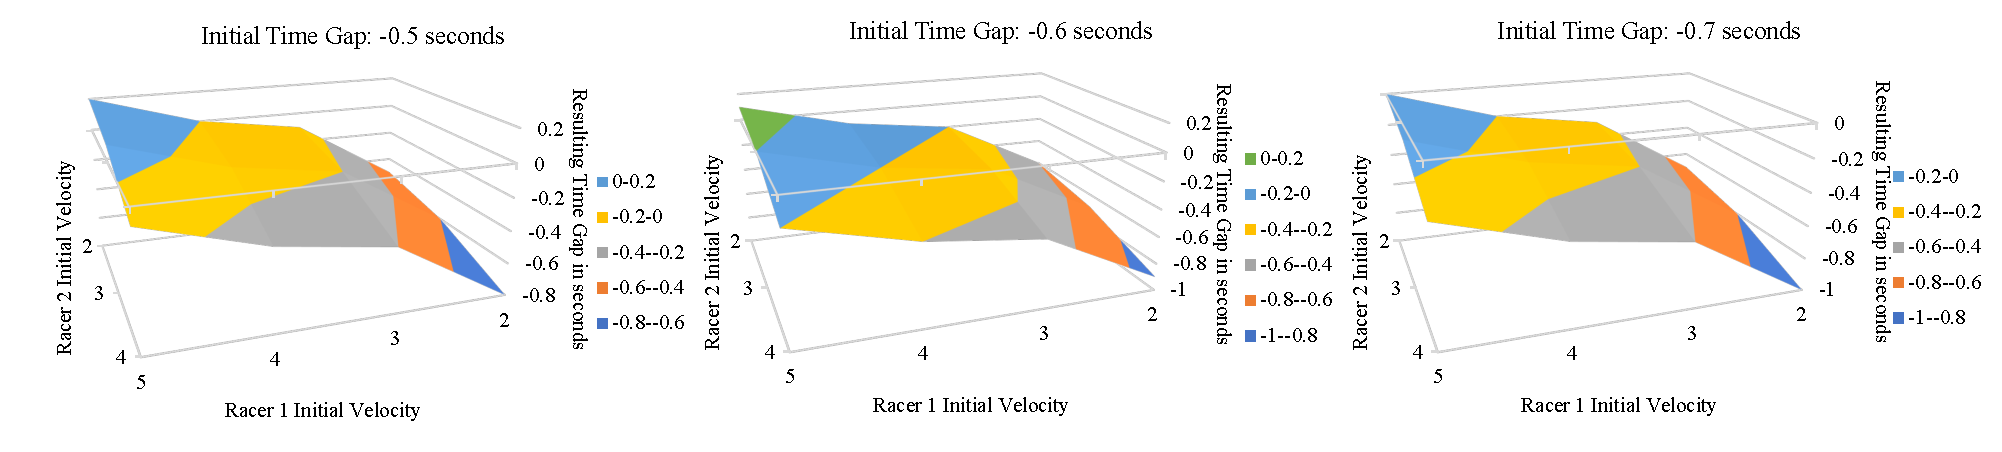
\includegraphics[width=\textwidth]{Figures/StraightExp.pdf}
    \caption[Results of scenarios in long straight case study.] { Plots for the resulting time gap by implementing both players' synthesized optimal strategy for various initial velocities and tire wear percentages in the long straight shape.}
    \label{fig:ls_exp}
\end{figure}

For each of the initial states we plot the resulting time gap assuming the players select their best action in Figure \ref{fig:ls_exp}. We observe a negative correlation between initial time disadvantage and the resulting time gap and a positive correlation between initial speed and the resulting time gap. Therefore, the results confirm that the model does meet the expected results based on the real-life understanding of where advantages are observed in this type of track shape. 
\begin{sidewaysfigure}
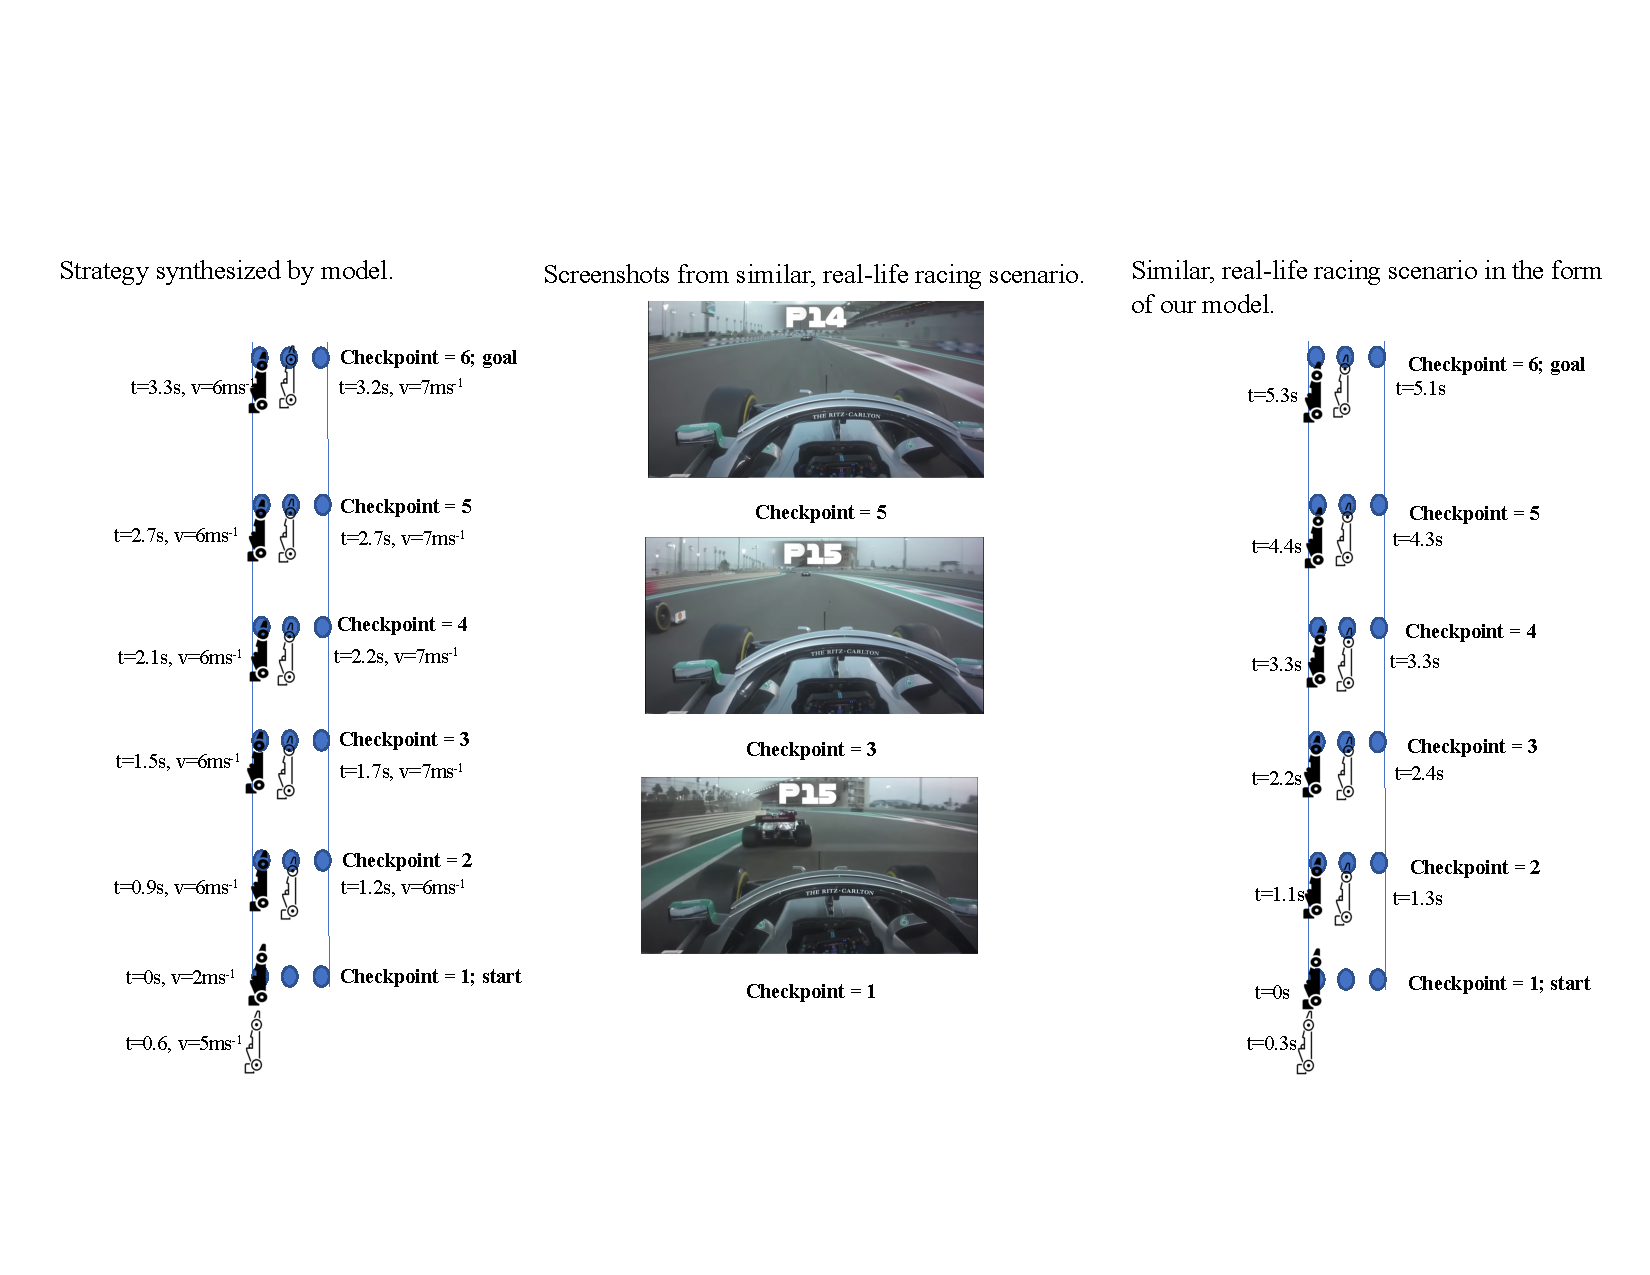
\includegraphics[height=0.8\textwidth, width=\textheight]{Figures/StraightViz.pdf}
    \caption[Synthesized strategy compared to real-life scenario on a long straight.] { Left: Visualized strategy synthesized in our case study scenario. Middle: Screenshots from a real-life race scenario resembling our case study.  Right: Extracted real race scenario represented in our model formulation.}
    \label{fig:ls}
\end{sidewaysfigure}
Next, we take a deeper dive in Figure \ref{fig:ls} by visualizing the players' strategies in one of the experiments. We show the specific scenario where the initial time disadvantage is \SI{0.6}{\second}, the initial velocity of racer 1 is \SI{5}{\meter\per\second} and the initial velocity of racer 2 is \SI{2}{\meter\per\second}. Player 1 and player 2 refer to the white car and black car, respectively. The synthesized strategy tells both cars to reach their top speeds, but it also indicates to player 1 to switch to the center lane. Player 1 is eventually able to build a \SI{0.1}{\second} time gap at the goal state due to its top speed advantage. The screenshots and the plotted real-life example\footnote{\label{straightnote}\url{https://youtu.be/z0tW3wY758Q?t=57}} is a straight section of the track that is about several hundred meters. While we don't know precise states of the players in the real-life video, we still use the video clip to plot the drivers' maneuvers using the time stamps. The tactic employed by the expert driver is similar to the one synthesized by the model in our case study. The driver switches to the center lane and uses the higher top speed and initial velocity to launch past the car that was originally in front. 

\FloatBarrier
% https://youtu.be/GxYzAqUs8N0?t=194
% https://youtu.be/64BQ-aXJkxA?t=28
% https://youtu.be/z0tW3wY758Q?t=57
\subsection{Hairpin}
 The second track shape is a hairpin turn, which is defined as a 180 degree turn. In reality, these types of turns generally follow long straights, but due state space explosion, the lead up to the hairpin turn is limited to just two checkpoints. Furthermore, because the turns are 180 degrees, the cars do not need to travel very fast. Therefore, having better acceleration and lower tire wear results in better performance in this type of track shape, and this pattern is seen in real-life races. In terms of strategy, the player that is initially ahead ideally positions itself in the middle of the straight approaching the turn to . Then, at the turn, the player wants to be at the innermost lane of the corner to force the opponent to take a wider turn or fall back in line. On the other hand, the player that is initially behind would like to reach the inside lane if at all possible and prevent the car that is ahead from using the inside lane. Tire wear begins to play an important role because it limits how tight of a turn is feasible for the players. Sometimes, the tire wear may be too high such that a player cannot use the inner most lane at the turn. Therefore, in the experiments for this scenario, we fix the initial time gap for racer 1 at 0.5 seconds but use varying combinations of initial velocities and tire wears for the racers. 

\begin{figure}[t!]
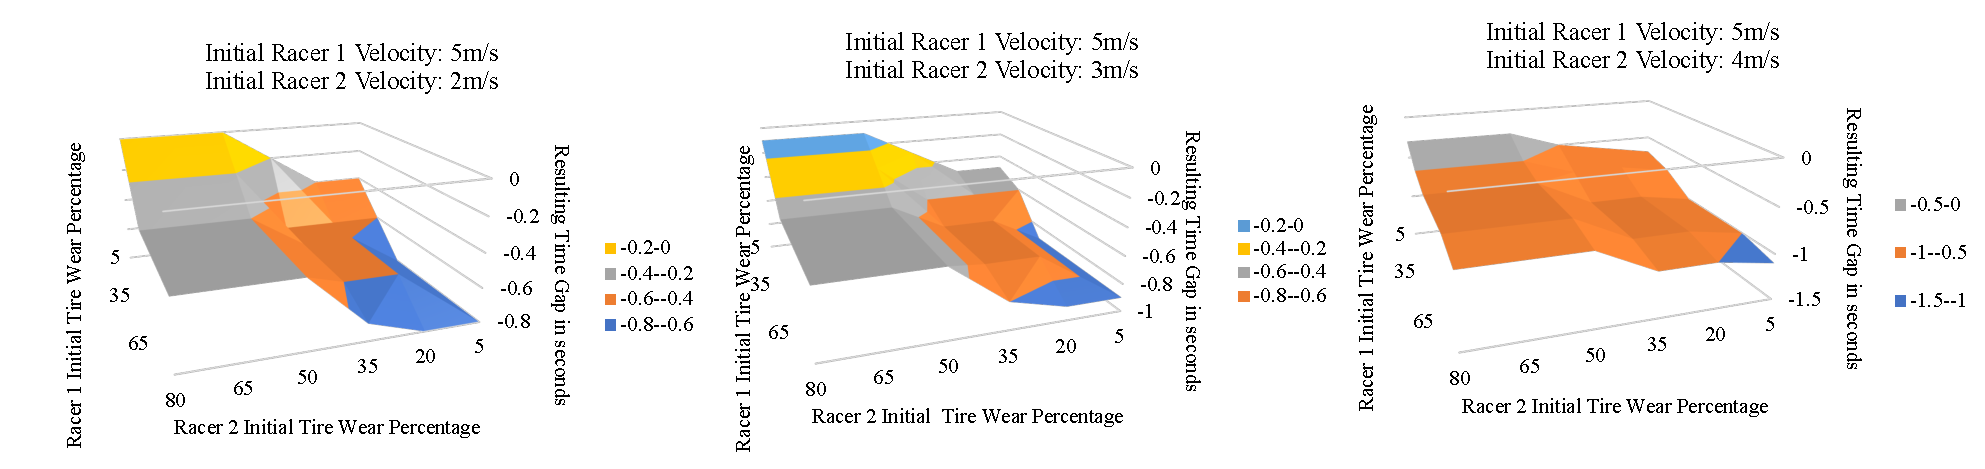
\includegraphics[width=\textwidth]{Figures/HairpinExp.pdf} 
    \caption[Results of scenarios in hairpin case study.] {Plots for the resulting time gap by implementing both players' synthesized optimal strategy for various initial velocities and tire wear percentages in the hairpin shape.}
    \label{fig:hp_exp}
\end{figure}

 In Figure \ref{fig:hp_exp}, we plot the results of our experiments. We see that player 2's higher acceleration allows it to stay ahead or only allow racer 1 to catch up but not pass despite having an initial velocity disadvantage. In other words, the player 1's time gap at the final checkpoint is always non-positive. The best case for player 1 is closing the time gap to 0 at the final checkpoint, and it occurs when player 2 is given a significant tire wear disadvantage. However, when there is a tire wear disadvantage for player 1, player 2 still maintained an advantage at the end despite having a lower initial velocity. These trends confirm that the model properly represents the advantages and disadvantages observed in real-life racing. 

\begin{sidewaysfigure}
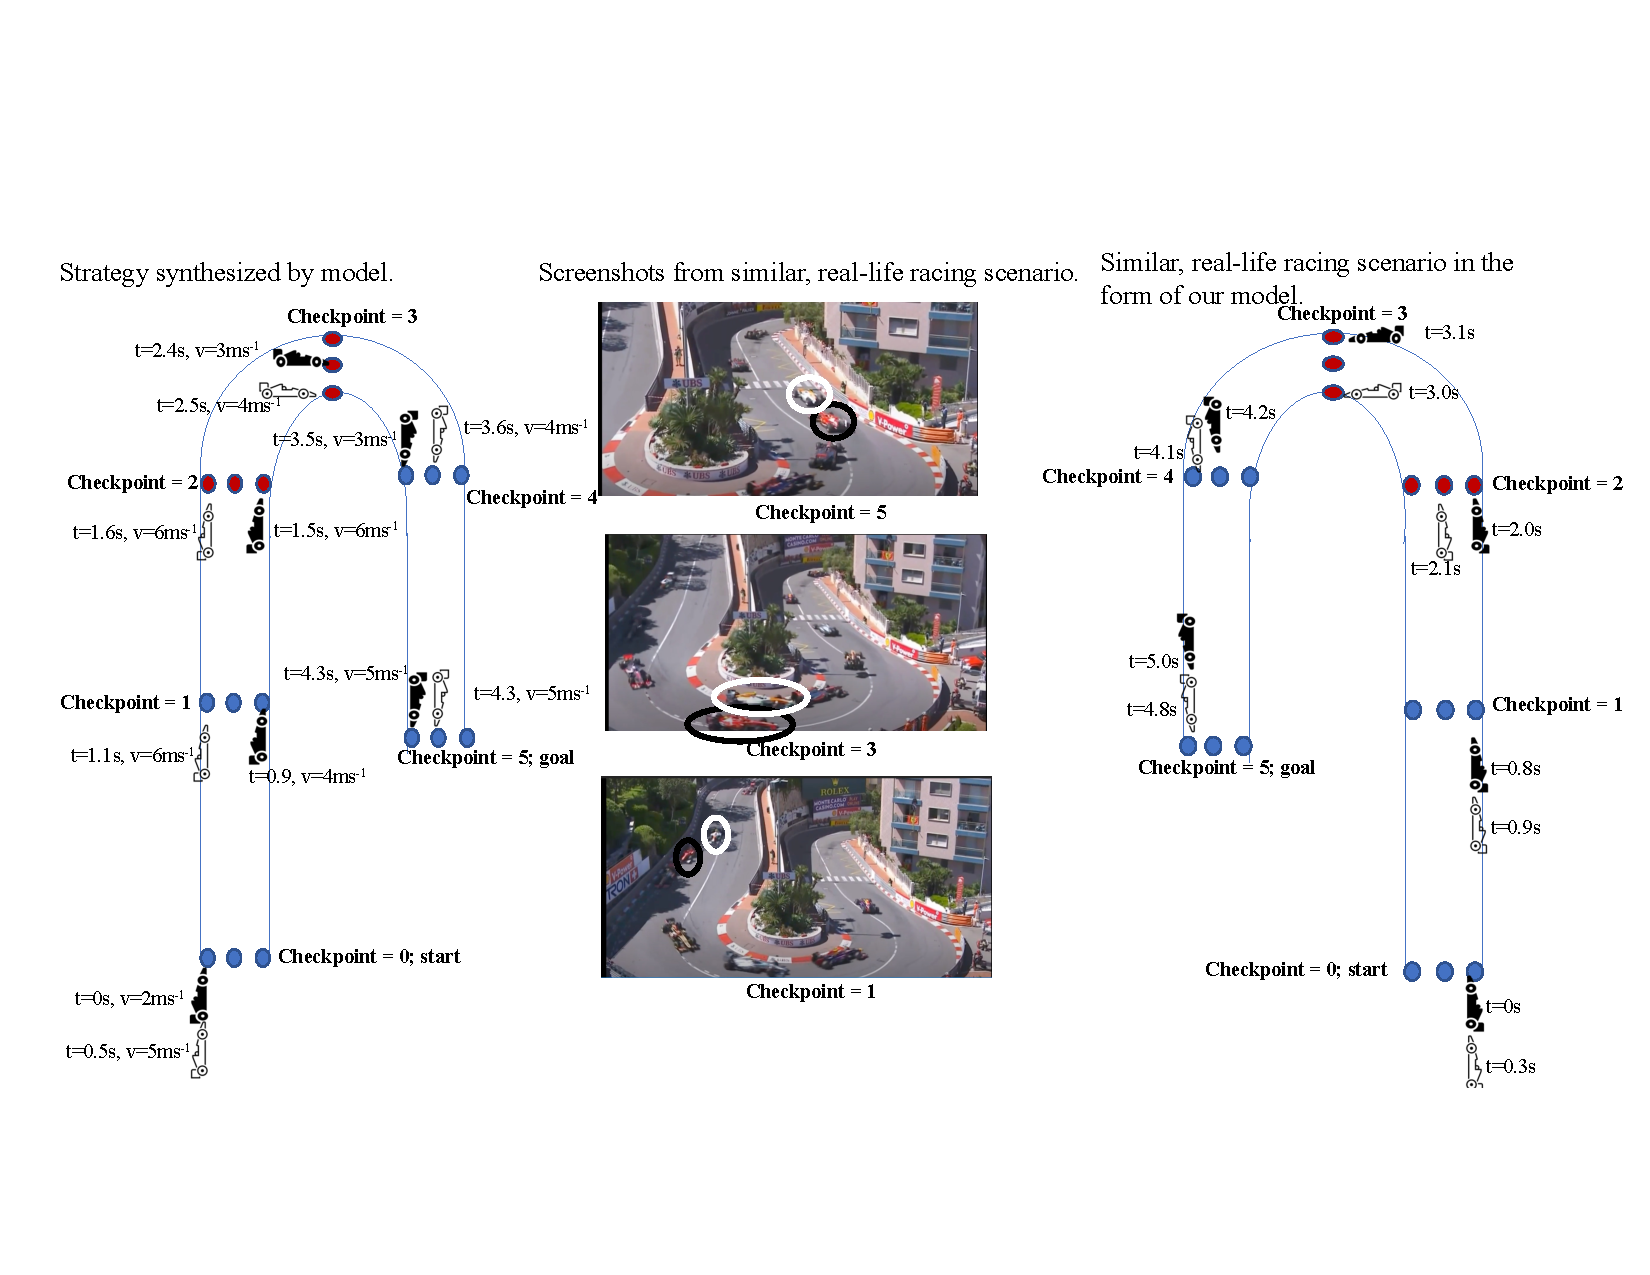
\includegraphics[height=0.8\textwidth, width=\textheight]{Figures/HairpinViz.pdf}
    \caption[Synthesized strategy compared to real-life scenario on a hairpin turn.] {Left: Visualized strategy synthesized in our case study scenario. Middle: Screenshots from a real F1 race.  Right: Extracted real race scenario represented in our model formulation.}
    \label{fig:hp}
\end{sidewaysfigure}

Next, we take a deeper dive in Figure \ref{fig:hp} to visualize the synthesized strategy from one of our scenarios. We study the scenario where player 1's initial velocity is 5 m/s, player 2's initial velocity is 2 m/s, player 1's initial tire age is 5\%, and player 2's initial tire age is 50\%. The screenshots from the real-life hairpin scenario\footnote{\label{hairpinnote}\url{https://youtu.be/CZdsBMhYnT4}} have other cars in the image, but the two main cars in question are circled in their respective colors matching the model extrapolation. Player 1 and player 2 refer to the white car and black car, respectively. In the synthesized model strategy, we see that player 2 immediately shifts over to the inner most lane to prevent any possible plan from the innermost lane because it knows that player 1 has both the tire age and speed advantage. However, player 2's state and dynamics prevent it from using the tightest lane in the turn due to its aged tires. As a result, it switches to the middle lane in the corner allowing player 1 to eventually choose the innermost lane. Upon the exiting the corner (from checkpoints 3 to 4), player 2 again chooses the inner most line because it is still ahead by \SI{0.1}{\second}. This choice forces player 1 use the wide lane and traverse a longer distance. As a result, player 1 is not able to overtake player 2, but it closes the gap to 0 seconds at the final position. This type of defensive maneuver of covering the inside lane, then going wide in the middle of the turn, and finally taking the inside on the exit of the turn is known as the ``switch-back'' in racing dialogue. The ``switch-back'' is commonly used by expert drivers because it sometimes catches the attacking driver off-guard. However, in the real-life video we compare to, we observe a slightly different strategy being executed. Player 1 passes player 2 because player 2 makes a sub-optimal choice and does not cover in the inside line at the hairpin. Rather, player 2 chooses to stay wide through out the turn allowing the fast approaching player 1 to take the inside lane at the corner and pass player 2 on the exit. 

% https://www.youtube.com/watch?v=CZdsBMhYnT4
\FloatBarrier
\subsection{Chicane}
 The final track shape is a chicane, which is a successive pair of turns of opposite direction (left-right or right-left). The chicane puts a greater emphasis on the tire wear than the prior two shapes, and success depends on the parameters of lateral force parameters of a player's vehicle. The inside of one turn is the outside of the following turn, so the racers must also have the low tire wear to maintain high speed over the shortest distance, which is hit the inside lane of both turns. Otherwise, compromising by selecting the middle lane may allow the other player to pass on the inside of one of the turns. In similar fashion to the hairpin case study experiments, we fix the initial time gap for player 1 at \SI{0.5}{\second} and use varying combinations of initial velocities and tire wears for these experiments.
 
 \begin{figure}[t!]
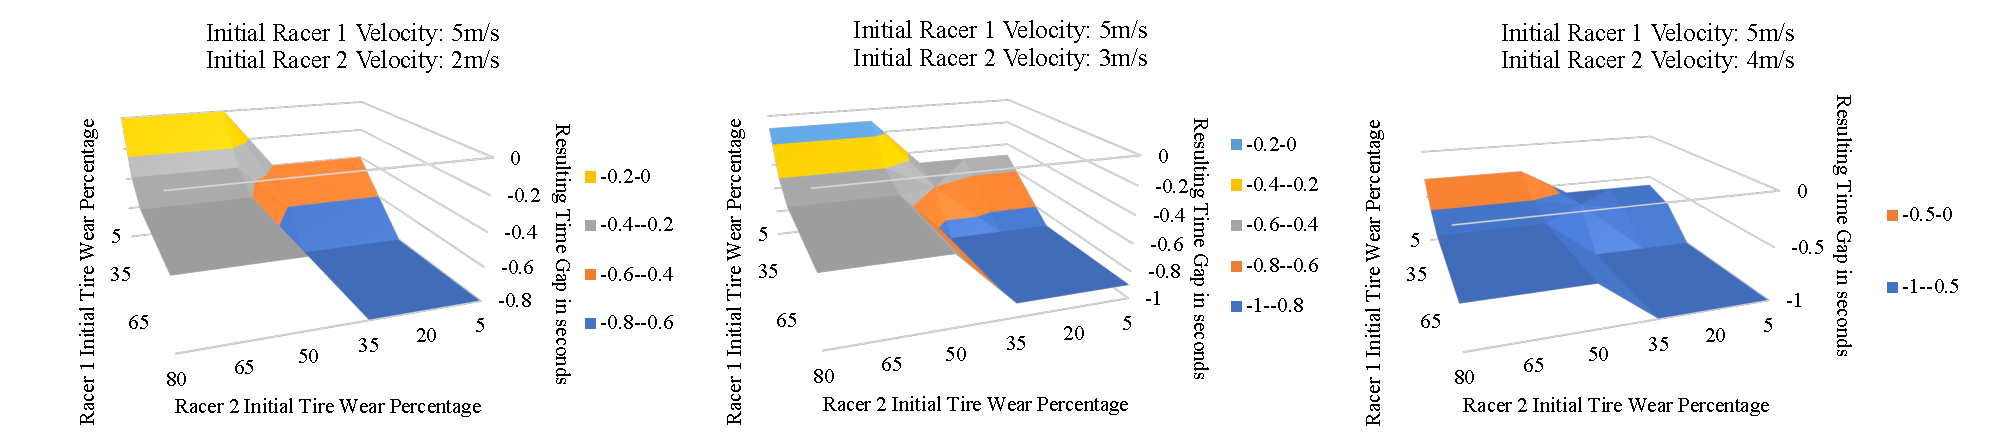
\includegraphics[width=\textwidth]{Figures/ChicaneExp.pdf}
    \caption[Results of scenarios in chicane case study.] {Plots for the resulting time gap by implementing both players' synthesized optimal strategy for various initial velocities and tire wear percentages in the chicane shape.}
    \label{fig:ch_exp}
\end{figure}
 
 Figure \ref{fig:ch_exp} shows a negative correlation between the final time gap between player 1 and player 2 and player 1's initial tire wear as expected. Furthermore, the lack of symmetry in surface of the plot shows the increased advantage for player 2 in some scenarios because it has a higher lateral acceleration limit. When the initial tire wear values are swapped for the racers, racer 2 maintains or builds on the initial \SI{0.5}{\second} time gap more often than racer 1 closes it. Again, the results indicate that model is a good representation of real-life racing because it follows the known patterns seen in real-life racing. 

\begin{sidewaysfigure}
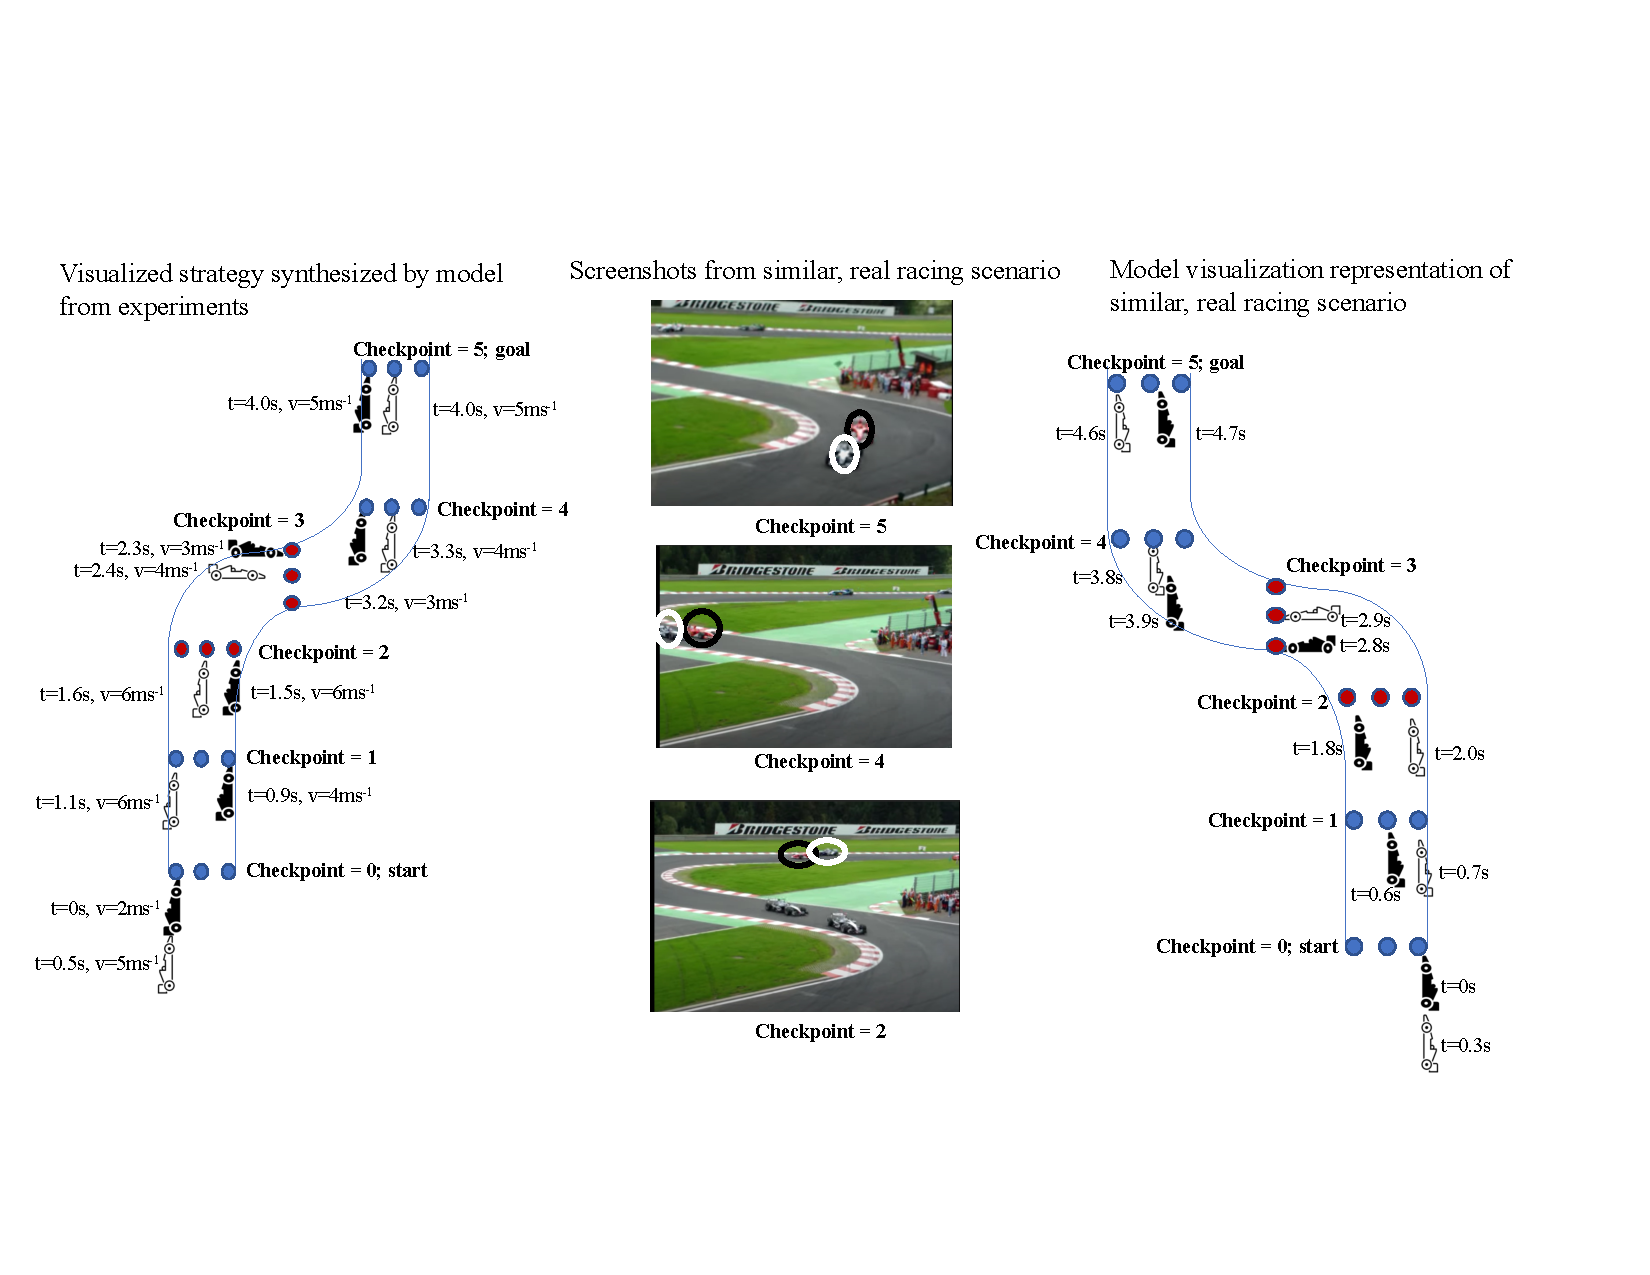
\includegraphics[height=0.8\textwidth, width=\textheight]{Figures/ChicaneViz.pdf}
    \caption[Synthesized strategy compared to real-life scenario on a chicane.]{Left: Visualized strategy synthesized in our case study scenario. Middle: Screenshots from a real F1 race. Right: Extracted real race scenario represented in our model formulation.}
    \label{fig:ch}
\end{sidewaysfigure}

In Figure \ref{fig:ch}, we visualize a synthesized strategy of one of the experiments over the chicane. We study the scenario where the the initial velocity of player 1 is \SI{5}{\meter\per\second}, the initial velocity of player 2 is \SI{2}{\meter\per\second}, the initial tire age of player 1 is 5\%, and the initial tire age of player 2 is 50\%. The screenshots from the real-life chicane scenario\footnote{\label{chicanenote}\url{https://youtu.be/_gWkHuOKR9w?t=6}} have the two main cars circled in their respective colors matching the model extrapolation. Player 1 and player 2 are the white and black cars, respectively. The synthesized strategy for this scenario presents a typical defensive maneuver where the initial leader, player 2, selects the inside line of both corners. This choice forces player 1 to use the wider line for both corners. However, player 1 has a lower tire wear and higher initial velocity, so he is able to improve the time gap and maintain a higher speed despite choosing the unfavorable line. As a result, initial time difference is reduced to \SI{0}{\second} at the final checkpoint. In the corresponding real-life scenario, we again observe a sub-optimal move by the leading human driver (in black) resulting in him being overtaken by the trailing driver (in white). The leading driver commits to the inside line for the first turn in the chicane, but stays wide on the second turn allowing the initially trailing driver to use the inside line at the second turn. As a result, the initially trailing driver has both the advantage of speed and shorter distance to travel with the inside line of the turn and makes the pass.  

\FloatBarrier
\section{Summary}
\begin{table}
\centering
\begin{tabular}{|l|l|p{4.5cm}|}
\hline
\textbf{Track Shape} & \textbf{Average Model Size} & \textbf{Average Time for Strategy Synthesis} 
\\ \hline
Straight   & 4200441 states      & \SI{394}{s}       \\ \hline
Hairpin   & 2139777  states     & \SI{200}{s}       \\ \hline
Chicane   & 2970922 states & \SI{273}{s}      \\ \hline
\end{tabular}%
\caption{Summary of model sizes and synthesis times for various track shapes.}
\label{table:discrete_exp_summary}
\end{table}
The results from the experiments show that our model provides a good representation of the prior understanding of advantage and disadvantage patterns in racing. We observe our discrete formulation and a state-of-the-art synthesis algorithm produce maneuvers that are comparable to those executed by professional human drivers while meeting the specification. In other words, the synthesized strategies follow all of the nuanced rules of racing while achieving the goal of reaching the target state before opponents or within the shortest time gap possible. In addition, we use these models to explain how the sub-optimal decisions of the human drivers in the real life-scenarios may have been corrected. The primary limitation of solving the discrete game formulation using formal methods is that it takes about 4 minutes, on average, to produce a result with various inputs we tested. Table \ref{table:discrete_exp_summary} summarizes the size of the game and average computation time. Therefore, we cannot directly use it for real-time control of an autonomous racecar suggesting we use probabilistic methods to approximate strategies.